% Template for ICIP-2013 paper; to be used with:
%          spconf.sty  - ICASSP/ICIP LaTeX style file, and
%          IEEEbib.bst - IEEE bibliography style file.
% --------------------------------------------------------------------------
\documentclass{article}

%%%%%%%%%%%%%%%%%%%%%
% My usual settings %
%%%%%%%%%%%%%%%%%%%%%
\usepackage{JB_config_article}
\usepackage{spconf}

%%%%%%%%%%%%%%%%%%%%%%%%%%%
% Location of the figures %
%%%%%%%%%%%%%%%%%%%%%%%%%%%
\graphicspath{{Images/}} 

% % Example definitions.
% % --------------------
% \def\x{{\mathbf x}}
% \def\L{{\cal L}}

% Title.
% ------
\title{SCATTERING HIDDEN MARKOV TREE}
%
% Single address.
% ---------------
\name{J.B. REGLI, J. D. B. NELSON \thanks{Thanks DSTL/UCL Impact studentship for funding.}}
\address{UCL, Department of statistical science}
%
% For example:
% ------------
%\address{School\\
%  Department\\
%  Address}
%
% Two addresses (uncomment and modify for two-address case).
% ----------------------------------------------------------
%\twoauthors
%  {A. Author-one, B. Author-two\sthanks{Thanks to XYZ agency for funding.}}
%  {School A-B\\
%  Department A-B\\
%  Address A-B}
%  {C. Author-three, D. Author-four\sthanks{The fourth author performed the work
%  while at ...}}
%  {School C-D\\
%  Department C-D\\
%  Address C-D}
%
\begin{document}
%\ninept
%
\maketitle
%
\begin{abstract}
  A Scattering convolutional hidden Markov tree proposes a new inference mechanism for high-dimensional signals by combining the interesting signal representation created by the scattering transform to a powerful probabilistic graphical model.
  A wavelet scattering network computes a signal translation invariant and stable to deformations representation that still preserves the informative content of the signal. Such properties are acquired by cascading wavelet transform convolutions with non-linear modulus and averaging operators.
  The network's structure and its distributions are described using a Hidden Markov Tree. This yield a generative model for high-dimensional inference. It offers a mean for performing several inference tasks among which are predictions. The scattering convolutional hidden Markov tree displays promising results on both classification and segmentation tasks of complex images.
\end{abstract}
%
\begin{keywords}
  Scattering network, Hidden Markov Model, Classification, Deep network
\end{keywords}
%
\section{Introduction}
\label{sec:Intro}

  The standard approach to classify high dimensional signals can be expressed as a two step procedure. First the data are projected in a feature space where the task at hand is simplified. Then prediction is done using a simple predictor in this new representational space. The mapping can either be hand-built ---\eg Fourier transform, wavelet transform--- or learned. In the last decade methods for learning the projection have drastically improved under the impulsion of the so called deep learning. Deep neural networks (sometime enriched by convolutional architecture) have been able to learn very effective representations for a given dataset and a given task~\citep{DNN, CNN}. Such method have achieved state of the art on many standard problems~\citep{alexNet} as well as real world applications~\citep{microsoft cortana}. 
  
%   Training those deep networks require an important number of training examples to be effective~\citep{training example in DNN}. Using    
%   ~\citep{one shot learning }
  
  %%%%%%%%%%%%%% =========== DUMMY TEXT =========== %%%%%%%%%%%%%%
  %TODO: change to highlight low number of training example properties 
  % From DL to one-shot learning + ST and WHMT
  Lorem ipsum dolor sit amet, consectetur adipiscing elit. Nulla pretium posuere auctor. Duis fermentum risus sit amet leo pretium dapibus. Integer a ligula iaculis, suscipit purus nec, malesuada dui. Morbi maximus mattis dolor, sed aliquam diam fermentum at. Fusce fringilla elementum pretium. Sed luctus nulla sit amet est tincidunt pellentesque volutpat id odio. Aenean accumsan ipsum eget velit feugiat, id rhoncus metus aliquet. Fusce vestibulum est id lorem ullamcorper, at iaculis tortor porttitor. Maecenas at ex nec tortor auctor efficitur.
  
  Etiam feugiat vel arcu eget efficitur. Quisque sed nisi nec nunc euismod sodales id eu elit. Sed dapibus interdum felis ut elementum. Maecenas vitae lacus commodo, consectetur nibh a, congue orci. Sed sit amet ipsum semper, imperdiet dolor vitae, pulvinar velit. Sed lorem massa, ornare eu sagittis in, vulputate ac nisl. In vel eros vel neque viverra mollis in sed velit. Nunc finibus magna nunc, eleifend vulputate ipsum iaculis non. Donec mollis sit amet diam ac vehicula. Vestibulum id enim mattis, ornare sapien non, mattis massa. Nulla quis gravida nisl. Integer varius dolor congue sem sagittis, non fermentum massa egestas. Nulla tempus aliquam sapien, in ultricies augue aliquam ac. Nunc et tincidunt felis, eget auctor odio. Aliquam posuere ut leo ut gravida. Fusce malesuada nisi eget tellus pulvinar, sed vulputate enim elementum.
  
  Sed rhoncus, ex vel vulputate eleifend, massa nisl egestas metus, a scelerisque nibh diam vel turpis. Nam pharetra arcu nec rutrum ullamcorper. Aenean lectus odio, mattis in efficitur eget, porttitor et sapien. Cras egestas libero nec nulla faucibus faucibus. Etiam vel enim venenatis mi aliquam efficitur at sit amet erat. Duis et aliquet ipsum, a elementum nisi. Aliquam convallis ligula odio, at bibendum libero tincidunt viverra. Vivamus bibendum molestie tortor, id varius eros laoreet ac. Curabitur quis neque ac erat elementum malesuada eget eget sem. Fusce vulputate nulla sit amet dolor convallis gravida. Nunc rutrum ultrices mi ac pellentesque. Mauris scelerisque pharetra sapien. Donec ultricies ex at neque blandit, finibus tempor libero eleifend. In at tellus diam. Morbi placerat magna nec dignissim sodales. Vivamus aliquam magna est, sed vehicula dolor dictum in. 
  %%%%%%%%%%%%%% =========== DUMMY TEXT =========== %%%%%%%%%%%%%%
  
%   We proposes a method combining a recently proposed deterministic analytically tractable transformation inspired by deep convolutional to a probabilistic graphical model in order to create a powerful probabilistic tool to handle high dimensional prediction problems. In a similar fashion to the work done by Crouse on wavelet trees~\citep{crouse1998wavelet}, we propose to describe Mallat's scattering convolutional scattering transform~\citep{bruna2010classification} using a hidden Markov tree. Doing so we develop a new framework to model high-dimensional inputs. As opposed to the commonly used simple classification method, once trained our model can tackle prediction problems but also other inference tasks ---\eg generation, sensitivity analysis... 

  In  Section~\ref{sec:Background}  we  present  the  requisite  background  of high dimensional signal classification. Section~\ref{sec:SCN} introduces the Scattering Transform and some of its properties.   We  fuse these to an hidden Markov Tree concepts in Section~\ref{sec:SCHMT}, propose our Scattering Hidden Markov Tree (SCHMT), and describe the inferential machinery. In Section~\ref{sec:Experiments} we perform classification on a selection of standard datasets. We draw conclusions in Section~\ref{sec:Conclusion}

  %TODO:
  % DL --- pb: not analytically tractable & lot of training examples required
  % ST --- pb: still require a few training examples
  % WHMT --- pb: not powerfull enough
  %Insist on the lot of training example needed for DL. Present ST has an alternative to lower the number of samples required.
  
  %Introduces Hidden Markov tree as an alternative to SVM providing generative model and better low proba perf

\section{Scattering networks}
  \label{sec:SCN}

%   Scattering convolutional networks (SCNs)~\citep{bruna} has the same general architecture as Convolutional Neural Networks (CNNs)~\citet{lecun1995convolutional}. They both cascade a convolution step and a ``pooling'' non linearity but CNNs use kernel filters learned from the data, while SCNs rely a fixed wavelet filter bank~\citep{mallat}. The wavelet bank can then be designed to extract image features having the desired invariant~\citep{work translation invariant, work rotation invariant, work rigid motion}. For image classification tasks, one is interested in producing descriptors that are ---at least--- stable to deformations and invariant to translation. Note that more while more complex SCNs exist, on the remainder of this paper we focus on descriptors with the previously mentioned properties.

    Scattering convolutional networks (SCNs)~\citep{bruna} are Convolutional Neural Networks (CNNs)~\citet{lecun1995convolutional} using a fixed filter bank of wavelets. Those filters can be hand-crafted to yield descriptors with the desired invariances~\citep{work translation invariant, work rotation invariant, work rigid motion}. For image classification tasks, one is interested in descriptors that are ---at least--- stable to deformations and invariant to translations. Note that SCNs producing more complexes set of invariances exist but on the remainder of this paper we consider only on descriptors with the previously mentioned properties.

  
  \subsection{Scattering transform}
    \label{subsec:SCN/ST}
    
    Wavelets are localized functions stable to deformations. They are thus well adapted to construct descriptor that would also be translation invariant. A two-dimensional spatial wavelet transform $W$ is obtained by scaling by $2^{j}$ and rotating by $r_{\theta}$ a mother wavelet $\psi$,
    \vspace{-5pt}
    \begin{equation}
      \label{eq:multi-scale directional wavelet}
      \psi_{\lambda}(u) = \psi_{j,\theta}(u) = 2^{-2j} \psi(2^{-j}r_{\theta}p)
    \end{equation}
    
    In the remainder of this paper we restrict to Morlet wavelet transforms defined on $\Lambda = G \times \llbracket 0,J \rrbracket$ where $G$ is a finite group of rotations of cardinal $L$ and where the wavelet is taken at scale $J$,
    \vspace{-5pt}
    \begin{equation}
      \label{eq:wavelet transform}
      W_{J}\bfx = \{ \bfx \ast \phi_{J}(u); \bfx \ast \psi_{\lambda}(u) \}_{p\in\dsR^{2},\lambda \in \Lambda}
    \end{equation}
    \vspace{-15pt}

    While the averaging part $\phi_{J}$ of the wavelet transform is invariant to translations, the high frequency part $\psi_{\lambda}$ is covariant to them~\citep{mallat}. Invariance within a limited range inferior $2^{J}$ can be achieved by averaging the positive envelope with a smooth window,
    \vspace{-5pt}
    \begin{equation}
      \label{eq:Scattering transform}
      S_{J}[\lambda]\bfx(u) = \abs{\bfx \ast \psi_{\lambda}} \ast \phi_{J}(u)
    \end{equation}
    \vspace{-10pt}
    
    Such non-linearised averaged wavelet coefficients are used in various form in computer vision (SIFT~\citep{sift}, DAISY~\citep{daisy}), but the scattering transform proposes a new non-linearity as well as a layer based architecture.
  
  \subsection{Scattering convolutional network}
    \label{subsec:SCN/SCN}
    
    While providing local translation invariance, the averaging convolution introduced in~\ref{eq:Scattering transform} also removes the spatial variability of the wavelet transform. SCNs cascade this wavelet modulus operator to recover the lost information and compute progressively more invariant descriptors. Let combine the wavelet transform and modulus operations into a single wavelet modulus operator,
    \vspace{-5pt}
    \begin{equation}
      \mcalU_{J} \bfx = \{ S[\emptyset] \bfx ; U[\lambda]\bfx \}_{\lambda \in \Lambda_{J}} 
          = \{ \bfx \ast \phi_{J}; \abs{\bfx \ast \psi_{\lambda}} \}_{\lambda \in \Lambda_{J}},
      \label{eq:One step propagator}
    \end{equation}
    
    A scattering transform can be interpreted as a CNN illustrated in Figure~\ref{fig:SCN 1}~\citep{Deep Roto-Translation Scattering for Object Classification} which propagates a signal $\bfx$ across multiple layers of the network and which outputs at each layer $m$ the scattering invariant coefficients $S[p_{m}]\bfx$ where $p_{m}=(\lambda_{1} \dots \lambda_{m})$ is a path of $m$ orientations and scales.
    
    \begin{figure}
      \begin{center}
        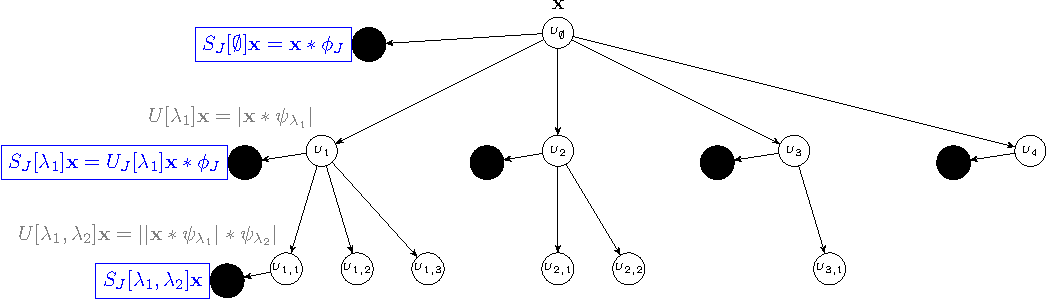
\includegraphics[width=3.3in, height=2in, keepaspectratio]{ST_freqDec_crop.pdf}
        \caption[Scattering convolution network.]{\centering  Scattering networks can be seen as neural networks iterating over wavelet  modulus  operators $\mcalU_{j}$. Each layer $m$ outputs the averaged  invariants $S[p_{m}]\bfx$ and covariant coefficients $U[p_{m+1}]\bfx$.}
        \label{fig:SCN 1}
        % TODO: Change it for something similar to Siffre rigid motion
      \end{center}
      \vspace{-15pt}
    \end{figure}
    
    The scattering energy is mainly concentrated along frequency decreasing paths, \ie for which $\abs{\lambda_{k+1}} \leq \abs{\lambda_{k}}$~\citep{mallat gis}. The energy contained in the other paths is negligible and thus for applications only frequency decreasing paths are considered. Moreover there exist a path length $M > 0$ after which all longer paths can be neglected. For signal processing applications, this decay appears to be exponential. And for classification applications, paths of length $M = 3$, \ie two convolutions, provides the most interesting results~\citep{anden2011multiscale},~\citep{bruna2010classification}.
      
    This restrictions yield an easier parametrization of a scattering network. Indeed its now completely defined by the mother wavelet $\phi$, the maximum path length considered $M$, the finest scale level considered $J$ and the number of orientation considered $L$.
      
    Hence for a given set of parameter $(\psi, M,J,L)$, let $ST_{(\psi, M,J,L)}(\bfx)$ denotes the unique frequency decreasing windowed scattering convolutional network with those parameters evaluated for signal $\bfx$. Each node $i$ of this network generates a -possibly empty- set of of nodes of size $(j_{i}-1) \times L$ where $j_{i}$ is the scale of node $i$ and $L$ is the number of orientations considered and it has the architecture displayed by Figure~\ref{fig:SCN 2}.

    \begin{figure}
      \begin{center}
        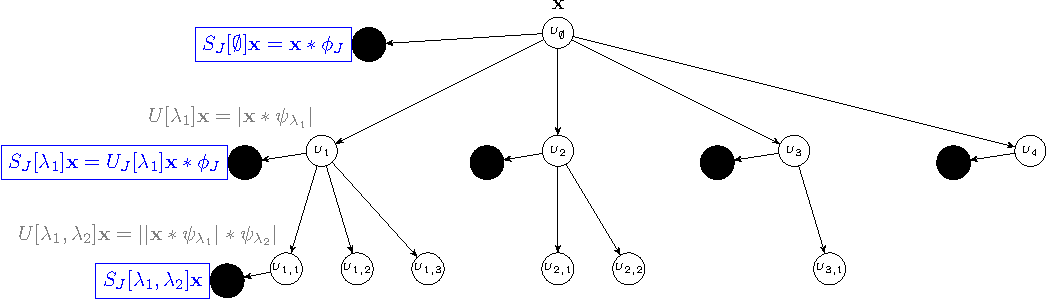
\includegraphics[width=3.3in, height=2in, keepaspectratio]{ST_freqDec_crop.pdf}
        \caption[Frequency decreasing scattering convolution network.]{\centering  Frequency decreasing scattering convolution network with $J=4$, $L=1$ and $M=2$. A node $i$ at scale $j_{i}$ generates $(j_{i}-1) \times L$ nodes. }
        \label{fig:SCN 2}
        % TODO: Narrow the gaps
      \end{center}
      \vspace{-15pt}
    \end{figure}
    
  \subsection{Scattering convolutional classifier}
    \label{subsec:SCN/SCC}
  
		In the original framework, the scattering network $ST_{(\psi, M,J,L)}(.)$ is used for classification task using a SVM classifier on the outputs of the network. Performance can be slightly improved by adding a feature selection step performing PCA on the scattering coefficients and keeping only the most informative ones. This classification framework provides results comparable with the state of the art on several datasets~\citep{bruna}.
    
    


% end of page 2

\section{The Scattering hidden Markov tree}
\label{sec:SCHMT}

  SCNs associated to a SVM classifier achieve good performance on classification task. However SVMs are not adapted to extremely limited number of training samples. They also provide only boolean labeling. The output of an SVM can be expressed as a probability~\citep{platt1999probabilistic} but it is a rescaling more than true probability. If one is interested in a true probabilistic models of the scattering coefficients, it is quite natural to express them as a probabilistic graphical model. We thus propose an adaptation of the wavelet hidden Markov trees~\citep{Crouse and Durand} to non-regular non-homogeneous tree structure of SCNs.
  
  \subsection{Hidden Markov tree model}
    \label{subsec:SCHMT/HMT model}
    %TODO Where to cite Crouse and Durand
        
    We model an SCN by a hidden Markov tree composed visible and hidden $\{\bfS_{i} , \bfH_{i}\}_{i \in \mcalT}$ nodes where $\forall i \in \mcalT$, $S_{i} \in \dsR$, $H_{i} \in \llbracket 1,K \rrbracket$ and $K$ is the number of hidden states. SCHMT models the correlation between scattering coefficients and there  through an hidden state.
    
    The initial state is drawn from a discrete non uniform distribution $\pi_{0}$ such that $\pi_{0}(k) = P(H_{0}=k)$.
    For any index $i$ of the tree, the emission distribution describes the probability of the visible node $S_{i}$ conditional to the hidden state $H_{i}$ and $P(S_{i}=s_{i}|H_{i}=k) = P_{\theta_{k,i}}(s)$ where $P_{\theta_{k,i}}$ belongs to a parametric distribution family and $\theta_{k,i}$ is the vector of emission parameters for the state $k$ and node $i$. In the remainder of the paper the emission distribution is Gaussian so that $P(S_{i}=s | H_{i}=k) = \mcalN(\mu_{k,i},\sigma_{k,i})$, where $\theta_{k,i}=(\mu_{k,i},\sigma_{k,i})$ with $\mu_{k,i}$ and $\sigma_{k,i}$ being respectively the mean and the variance of the Gaussian for the $k$-th value of the mixture and the node $i$.
    Finally the probability for the hidden node $H_{i}$ to be in a state $k$ given its father's state $g$ is characterized by a transition probability such that $\epsilon_{i}^{(gk)} = P(H_{i}= k | H_{\rho(i)}=g)$ where $\epsilon_{i}$ defines a transition probability matrix such that $P(H_{i}=k) = \sum_{g=1}^{K} \epsilon_{i}^{(gk)} P(H_{\rho(i)}=g)$.
    %TODO: find this formula in Durand article

    Such a model is pictured in Figure~\ref{fig:SCHMT 1} and for a given scattering architecture ---\ie fixed $M$, $J$ and $L$--- the SCHMT model is fully parametrized by,
    \vspace{-5pt}
    \begin{equation}
      \Theta = \big(\pi_{0}, \{ \epsilon_{i}, \{ \theta_{k,i} \}_{k\in\llbracket1,K\rrbracket} \}_{i\in\mcalT}\big).
      \label{eq:SCHMT - parameters}
    \end{equation}
    \vspace{-15pt}

    \begin{figure}
      \begin{center}
        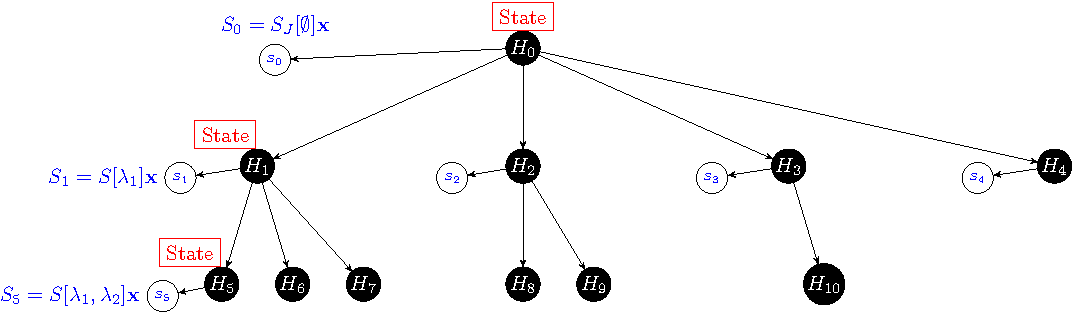
\includegraphics[width=3.3in, height=2in, keepaspectratio]{scat_HMT_crop.pdf}
        \caption{Scattering convolutional hidden Markov tree.}
        \label{fig:SCHMT 1}
        % TODO: Narrow the gaps
      \end{center}
    \end{figure}

    This model implies to do two assumptions on the scattering transform. First one need to assume --- $K$-populations--- that a signal’s scattering coefficients can be described by K clusters. This is a common assumptions for standard wavelets~\citep{kingsbury2001complex} and hence it can be extended to the scattering transform. The SCHMT also assumed ---persistence--- that the informative character of a coefficients is propagated across layers. This assumption is sound since scattering coefficients are highly correlated across layers~\citep{Oyallon}.
    
  \subsection{Learning the tree parameters}
    \label{subsec:SCHMT/Learning}    

    The SCHMT is trained using the smoothed version of the Expectation-Maximization (EM) algorithm \citep{someone} for hidden Markov trees proposed by~\citep{Durand} and adapted to non-homogeneous and non-binary trees.
    
    The smoothed version of the E-step requires the computation of the conditional probability distributions $\xi_{i}(k) = P(H_{i}=k | \bar{\mcalS}_{i}= \bar{s}_{i})$ (smoothed probability) and $P(H_{i}=k, H_{\rho(i)}=g | \bar{\mcalS}_{i}= \bar{s}_{i})$ for each node $i \in \mcalT$ and states $k$ and $g$. This can be achieved through an upward-downward recursion displayed in Algorithm~\ref{algo:Smoothed upward} and~\ref{algo:Smoothed downward}.
    \vspace{-20pt}
    \setlength{\algomargin}{+4pt}
    \begin{center}
      \begin{algorithm}
	\vspace{-3pt}
	\fontsize{8pt}{10pt}\selectfont
%          \textbf{Meta-parameters:}\\
%         $K$\\
        \tcp{Initialization:}
%         \tcp{$P_{\theta_{k,i}}(s_{i})$:}
        \For{All the nodes $i$ of the tree $\mcalT$}{ 
          $P_{\theta_{k,i}}(s_{i}) = \mcalN(s_{i} | \mu_{k,i},\sigma_{k,i})$
        }
%         \tcp{Loop over the leaves $i$ of the tree:}
        \For{All the leaves $i$ of the tree $\mcalT$}{
          $\beta_{i}(k) = \frac{P_{\theta_{k,i}}(s_{i}) P(H_{i}=k)}{\sum_{g=1}^{K} P_{\theta_{g,i}}(s_{i}) P(H_{i}=g)}$\\
          $\beta_{i,\rho(i)}(k) = \sum_{g=1}^{K}\frac{\beta_{i}(g) \epsilon_{i}^{(kg)}}{P(H_{i}=g)} . P(H_{\rho(i)}=k)$ \\
          $l_{i} = 0$
        }
        \tcp{Induction:}
%         \tcp{Bottom-Up loop over the nodes of the tree:}
        \For{All non-leaf nodes $i$ of the tree $\mcalT$ (Bottom-up)}{
          $M_{i} = \sum_{k=1}^{K} P_{\theta_{k,i}}(s_{i}) \prod_{j \in c(i)} \frac{\beta_{j,i}(k)}{P(H_{i}=k)^{n_{i}-1}}$ \\
          $l_{i} = \log(M_{i}) + \sum_{j \in c(i)}l_{j}$\\
          $\beta_{i}(k) = \frac{P_{\theta_{k,i}(s_{i})} \prod_{j \in c(i)}(\beta_{j,i}(k))}{P(H_{i}=k) ^{n_{i}-1} M_{i}} $\\
          \For{All the children nodes $j$ of node $i$}{
            $\beta_{i\backslash c(i)}(k) = \frac{\beta_{i}(k)}{\beta_{i,j}(k)}$
          }
          $\beta_{i,\rho(i)}(k) = \sum_{g=1}^{K} \frac{\beta_{i}(g) \epsilon_{i}^{(kg)}}{P(H_{i}=g)} .P(H_{\rho(i)}=k)$
        }
        \caption{Smoothed upward algorithm.}
        \label{algo:Smoothed upward}
        \vspace{-5pt}
      \end{algorithm}        
    \end{center}
    \vspace{-30pt}
    \vspace{-20pt}  
    \begin{center}
      \begin{algorithm}
	\vspace{-3pt}
	\fontsize{8pt}{10pt}\selectfont
%         \textbf{Meta-parameters:}\\
%         $K$\\
        \tcp{Initialization:}
        $\alpha_{0}(k) = 1$\\
        \tcp{Induction:}
%         \tcp{Top-Down loop over the nodes of the tree:}
        \For{All nodes $i$ of the tree $\mcalT\backslash\{0\}$ (Top-Down)}{
          $\alpha_{i}(k) = \frac{1}{P(H_{i}=k)} \sum_{g=1}^{K} \alpha_{\rho(i)}(g) \epsilon_{i}^{(gk)} \beta_{\rho(i)\backslash i}(g) P(H_{\rho(i)}=g)$
        }
        \caption{Smoothed downward algorithm.}
        \label{algo:Smoothed downward}  
	\vspace{-5pt}
      \end{algorithm}        
    \end{center}
    \vspace{-30pt}
    \vspace{-20pt}  
    \begin{center}
      \begin{algorithm}
	\vspace{-3pt}
	\fontsize{8pt}{10pt}\selectfont

%         \textbf{Meta-parameters:}\\
%         $K$,\\
%         Distribution family for $P_{\theta}$ \tcp*{Here Gaussian}
%         $N$ \tcp*{Number of observed realizations of the signal}
        \tcp{Initialization:}
        $\pi_{0}(k) = \frac{1}{N} \sum_{n=1}^{N} P(H_{0}^{n}=m|s_{0}^{n},\Theta^{l})$\\
        \tcp{Induction:}
%         \tcp{Loop over the nodes of the tree:}
        \For{All nodes $i$ of the tree $\mcalT\backslash\{0\}$}{
          $P(H_{i}=k) = \frac{1}{N} \sum_{n=1}^{N} P(H_{i}^{n}=k|\bar{s}_{0}^{n},\Theta^{l})$,\\
          $\epsilon_{i}^{gk} = \frac{\sum_{n=1}^{N} P(H_{i}^{n} = k, H_{\rho(i)}^{n}=g |\bar{s}_{0}^{n}, \Theta^{l})} {N P(H_{\rho(i)}=k)}$,\\
          $\mu_{k,i} = \frac{\sum_{n=1}^{N} s_{i}^{n} P(H_{i}^{n} = k |\bar{s}_{0}^{n}, \Theta^{l})} {N P(H_{i}=k)}$,\\
          $\sigma_{k,i}^{2} = \frac{\sum_{n=1}^{N} (s_{i}^{n} - \mu_{k,i})^{2} P(H_{i}^{n} = k |\bar{s}_{0}^{n}, \Theta^{l})} {N P(H_{i}=k)}$.
        }
        \caption{M-step of the EM algorithm.}
        \label{algo:Mstep}
	\vspace{-5pt}
      \end{algorithm}        
    \end{center}
    
\section{Classification results}
  \label{sec:Experiments}


\section{Conclusion}
  \label{sec:Conlusion}




% Below is an example of how to insert images. Delete the ``\vspace'' line,
% uncomment the preceding line ``\centerline...'' and replace ``imageX.ps''
% with a suitable PostScript file name.
% -------------------------------------------------------------------------
% \begin{figure}[htb]
%   \begin{minipage}[b]{1.0\linewidth}
%     \centering
%     \centerline{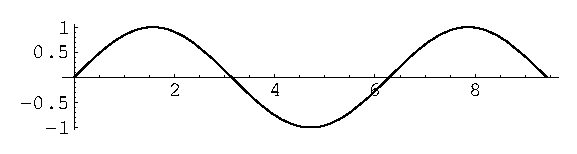
\includegraphics[width=8.5cm]{image1}}
% %   \vspace{2.0cm}
%     \centerline{(a) Result 1}\medskip
%   \end{minipage}
% %
%   \begin{minipage}[b]{.48\linewidth}
%     \centering
%     \centerline{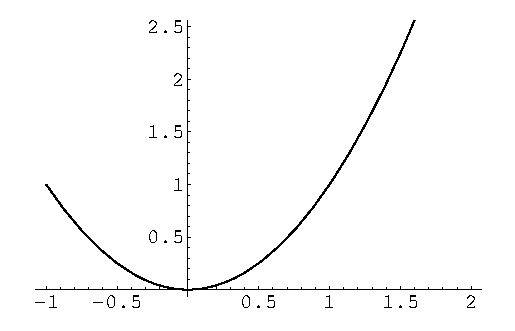
\includegraphics[width=4.0cm]{image3}}
% %   \vspace{1.5cm}
%     \centerline{(b) Results 3}\medskip
%   \end{minipage}
%   \hfill
%   \begin{minipage}[b]{0.48\linewidth}
%     \centering
%     \centerline{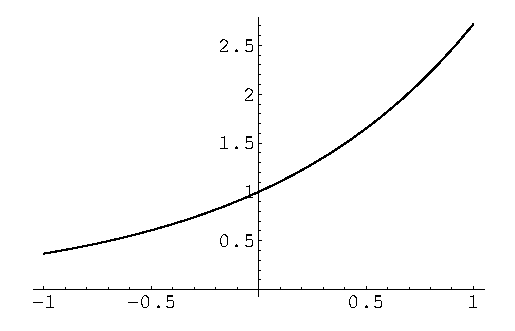
\includegraphics[width=4.0cm]{image4}}
% %   \vspace{1.5cm}
%     \centerline{(c) Result 4}\medskip
%   \end{minipage}
% %
%   \caption{Example of placing a figure with experimental results.}
%   \label{fig:res}
% \end{figure}


% To start a new column (but not a new page) and help balance the last-page
% column length use \vfill\pagebreak.
% -------------------------------------------------------------------------
\vfill
\pagebreak

\section{COPYRIGHT FORMS}
\l1abel{sec:copyright}

You must include your fully completed, signed IEEE copyright release form when
form when you submit your paper. We {\bf must} have this form before your paper
can be published in the proceedings.

\section{REFERENCES}
\label{sec:ref}
  


% References should be produced using the bibtex program from suitable
% BiBTeX files (here: strings, refs, manuals). The IEEEbib.bst bibliography
% style file from IEEE produces unsorted bibliography list.
% -------------------------------------------------------------------------
\bibliographystyle{IEEEbib}
%\bibliography{strings,refs}
% \bibliography{bib_icip}

\end{document}
